\documentclass[11pt,a4paper]{article}
\usepackage[utf8]{inputenc}
\usepackage[T1]{fontenc}
\usepackage{amsthm} %numéroter les questions
\usepackage[frenchb]{babel}
\usepackage{datetime}
\usepackage{xspace} % typographie IN
\usepackage{hyperref}% hyperliens
\usepackage[all]{hypcap} %lien pointe en haut des figures
\usepackage[french]{varioref} %voir x p y
\usepackage{fancyhdr}% en têtes
%\input cyracc.def
\usepackage[]{graphicx} %include pictures
\usepackage{pgfplots}
\usepackage[]{circuitikz}
\usepackage{ifthen}

\usepackage[top=1.3 in, bottom=1.3 in, left=1.3 in, right=1.3 in]{geometry} % Yeah, that's bad to play with margins
\usepackage[]{pdfpages}

\usepackage[]{attachfile}

\usepackage{float}
\usepackage{subfig}

\usepackage{todonotes} % \missingfigure
\usepackage{gensymb} % \ohm

\usepackage{framed}

\newdateformat{mydate}{v1.0.1}%hack pour remplacer \THEYEAR


\newboolean{corrige}
\ifx\correction\undefined
\setboolean{corrige}{false}% pas de corrigé
\else
\setboolean{corrige}{true}%corrigé
\fi

%\setboolean{corrige}{false}% pas de corrigé

\newboolean{annexes}
\setboolean{annexes}{true}%annexes
%\setboolean{annexes}{false}% pas de annexes

\definecolor{darkblue}{rgb}{0,0,0.5}

\newboolean{mos}
%\setboolean{mos}{true}%annexes
\setboolean{mos}{false}% pas de annexes

\usepackage{aeguill} %guillemets

%% fancy header & foot
\pagestyle{fancy}
%Numero du TP :
\def \labonumber {Project specifications}
\lhead{[ELEC-H-310] Choucroute numérique\\ \labonumber}
\rhead{\mydate\today\\ page \thepage}
\chead{\ifthenelse{\boolean{corrige}}{Corrigé}{}}
\cfoot{}
%%

\pdfinfo{
/Author (Quentin Delhaye, Ken Hasselmann, ULB -- BEAMS)
/Title (\labonumber ELEC-H-310)
/ModDate (D:\pdfdate)
}

\hypersetup{
pdftitle={\labonumber [ELEC-H-310] Choucroute numérique},
pdfauthor={Quentin Delhaye, Ken Hasselmann, ULB -- BEAMS},
pdfsubject={}
}

\theoremstyle{definition}% questions pas en italique
\newtheorem{Q}{Question}[] % numéroter les questions [section] ou non []

\newcommand{\reponse}[1]{% pour intégrer une réponse : \reponse{texte} : sera inclus si \boolean{corrige}
	\ifthenelse {\boolean{corrige}} {\paragraph{Réponse :} \color{darkblue}   #1\color{black}} {}
 }

\newcommand{\addcontentslinenono}[4]{\addtocontents{#1}{\protect\contentsline{#2}{#3}{#4}{}}}

\date{\vspace{-1.7cm}\mydate\today}
\title{\vspace{-2cm} \labonumber\\ Digital electronics [ELEC-H-310]\\Design of a temperature regulation system\ifthenelse{\boolean{corrige}}{~\\Corrigé}{}}

%\author{\vspace{-1cm}}%\textsc{Yannick Allard}}

\setlength{\parskip}{0.2cm plus2mm minus1mm} %espacement entre §
\setlength{\parindent}{0pt}






%%%%%%%%%%%%%%%%%%%%%%%%%%%%%%%%%%%%%%%%%%%%%%%%%%%%%%%%%%%%%%%%%%%%%%%%%%%%%%%%%%%%%%%%%%%%%%%%%%%%%%%%%%%%%
%%%%%%%%%%%%%%%%%%%%%%%%%%%%%%%%%%%%%%%%%%%%%%%%%%%%%%%%%%%%%%%%%%%%%%%%%%%%%%%%%%%%%%%%%%%%%%%%%%%%%%%%%%%%%
%%%%%%%%%%%%%%%%%%%%%%%%%%%%%%%%%%%%%%%%%%%%%%%%%%%%%%%%%%%%%%%%%%%%%%%%%%%%%%%%%%%%%%%%%%%%%%%%%%%%%%%%%%%%%
% http://tex.stackexchange.com/questions/128123/circuitikz-current-source
% preparation to create bipoles

\makeatletter
\def\TikzBipolePath#1#2{\pgf@circ@bipole@path{#1}{#2}}

%\pgf@circ@Rlen = \pgfkeysvalueof{/tikz/circuitikz/bipoles/length}
\makeatother

\newlength{\ResUp} \newlength{\ResDown}
\newlength{\ResLeft} \newlength{\ResRight}

% set default dohicky size

\ctikzset{bipoles/doohicky/height/.initial=.4}
\ctikzset{bipoles/doohicky/width/.initial=.6}

% create doohicky shape

\pgfcircdeclarebipole{}
 {\ctikzvalof{bipoles/doohicky/height}}
 {doohicky}
 {\ctikzvalof{bipoles/doohicky/height}}
 {\ctikzvalof{bipoles/doohicky/width}}
 {
    \pgfsetlinewidth{\pgfkeysvalueof{/tikz/circuitikz/bipoles/thickness}\pgfstartlinewidth}
    \pgfextractx{\ResRight}{\northeast}
    \pgfextracty{\ResUp}{\northeast}
    \pgfextractx{\ResLeft}{\southwest}

  \pgfmoveto{\pgfpoint{\ResLeft}{0cm}}
    \pgfpathellipse{\pgfpoint{0.333\ResLeft}{0cm}}{\pgfpoint{0.667\ResRight}{0cm}}{\pgfpoint{0cm}{\ResUp}}
  \pgfmoveto{\pgfpoint{\ResRight}{0cm}}
    \pgfpathellipse{\pgfpoint{0.333\ResRight}{0cm}}{\pgfpoint{0.667\ResRight}{0cm}}{\pgfpoint{0cm}{\ResUp}}
  \pgfusepath{draw} %draw doohicky
    \pgfscope
    \pgfsetarrowsend{latex'}
    \pgfpathmoveto{\pgfpoint{0.667\ResLeft}{1.333\ResUp}}
    \pgfpathlineto{\pgfpoint{0.667\ResRight}{1.333\ResUp}}
    \pgfusepath{draw}   %draw arrow
    \endpgfscope
 }

% create doohicky to-path style

\def\doohickypath#1{\TikzBipolePath{doohicky}{#1}}
\tikzset{doohicky/.style = {\circuitikzbasekey, /tikz/to path=\doohickypath, l=#1}}

% end of setup
%%%%%%%%%%%%%%%%%%%%%%%%%%%%%%%%%%%%%%%%%%%%%%%%%%%%%%%%%%%%%%%%%%%%%%%%%%%%%%%%%%%%%%%%%%%%%%%%%%%%%%%%%%%%
%%%%%%%%%%%%%%%%%%%%%%%%%%%%%%%%%%%%%%%%%%%%%%%%%%%%%%%%%%%%%%%%%%%%%%%%%%%%%%%%%%%%%%%%%%%%%%%%%%%%%%%%%%%%
%%%%%%%%%%%%%%%%%%%%%%%%%%%%%%%%%%%%%%%%%%%%%%%%%%%%%%%%%%%%%%%%%%%%%%%%%%%%%%%%%%%%%%%%%%%%%%%%%%%%%%%%%%%%





















\begin{document}
\pagestyle{empty}
\maketitle
% \vspace*{-1cm}


% ########   ##      ##  ##########  ########     #####
%    ##      ###     ##      ##      ##     ##  ##     ##
%    ##      ## ##   ##      ##      ##     ##  ##     ##
%    ##      ##  ##  ##      ##      ########   ##     ##
%    ##      ##   ## ##      ##      ##   ##    ##     ##
%    ##      ##     ###      ##      ##    ##   ##     ##
% ########   ##      ##      ##      ##     ##    #####

\section{Introduction}
The aim of the project is to design a temperature regulation system similar to those used in laptops.
Thanks to the airflow generated by a variable speed fan, the processor temperature is kept cooled in the imposed limits despite its power fluctuations.

\begin{center}
\begin{figure}[H]
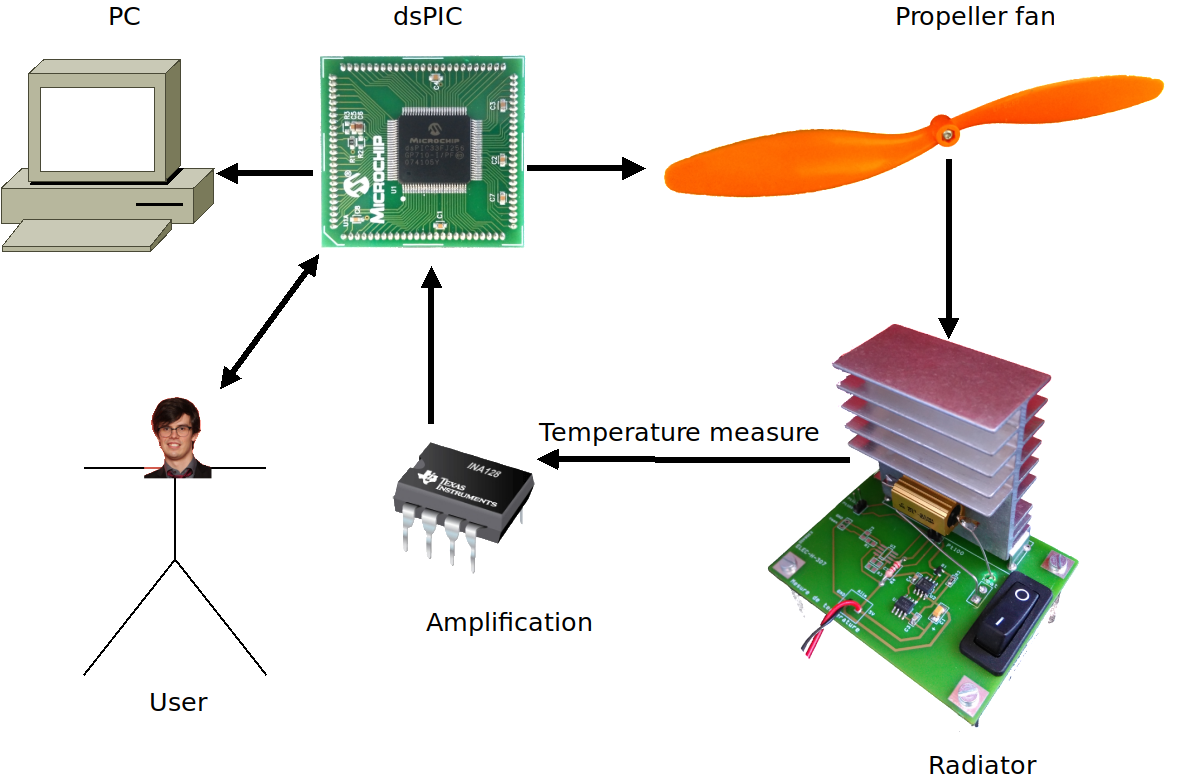
\includegraphics[width=\textwidth]{workflow}
\caption{Project diagram}
\label{fig:workflow}
\end{figure}
\end{center}

In this project, you will dispose of~:
\begin{itemize}
	\item An Explorer 16 board with a dsPIC33.
	\item A propeller driven by;
	\item A DC motor which will act as a fan.
	\item A temperature probe.
	\item A heating resistor mounted on a heat sink which will act as the processor.
	\item A keyboard.
	\item A LCD screen.
	\item A serial connection with a computer making possible to prompt the temperature evolution through time.
\end{itemize}




%  #######      ###     ##     ##  ########   #########  ########
% ##     ##    ## ##    ##     ##     ##      ##         ##     ##
% ##          ##   ##   ##     ##     ##      ##         ##     ##
% ##         ##     ##  #########     ##      ######     ########
% ##         #########  ##     ##     ##      ##         ##   ##
% ##     ##  ##     ##  ##     ##     ##      ##         ##    ##
%  #######   ##     ##  ##     ##  ########   #########  ##     ##



\section{Project specifications}
The project is relatively complex, we will describe the requirements here.

The cooling of the heating resistor is made by rotating the propeller at variable speed. 
You will need to control the power that will be delivered to the DC motor.

Similarly to the ELEC-H-301 labs, the power amplifier powering the motor is controlled by a PWM square wave (see section~\ref{sec:helice}).
Therefore, you will have to design a system to generate adjustable square waves.
The period of the square wave should be short compared with the mechanical time constant of the motor (its rotational speed should be almost constant during a PWM period).

By measuring the heating resistor temperature and adjusting motor speed, you will be able to design a closed-loop regulation.
You may implement a very simple regulation procedure such as a proportional regulator. 
If you want you may implement more complex algorithms (PI, PID, ...) but this is optional.

\begin{center}
\framebox{\quad In regime, the temperature static error should be inferior to $1\celsius$ \quad}
\end{center}

The temperature is made with a platinum resistor of the type Pt100. 
Those resistors vary linearly with the temperature using the law $R(T) = 100\ohm + \alpha T$, where $\alpha = 0.385\ohm/\celsius$ ($T$ is in Celsius).
By keeping the current constant, it becomes possible to deduce temperature from a measure of its tension.
The complete acquisition circuit is describe later.

\begin{center}
\framebox{\quad We suppose that the temperature will not be superior to $45\celsius$ \quad}
\end{center}

The user must be able to operate the system by interacting with the keyboard and the LCD screen present on the expansion board.
Here are the operationnal commands~:
\begin{itemize}
	\item Touch 'A' + two digits~: changes the temperature command.
	Example~: «~A23~» sets the desired temperature to $23\celsius$.
	\item Touch 'B' + two digits~: changes the sampling period.
	Example~: «~B0250~» sets the periode to $250\ ms$.
	It should accept periods in a $1\ ms$ to $1\ s$ range.
	\item Touch 'F': acts as the enter key. 
	\item Touch 'C': deletes the last character entered.
	\item Touch 'D': cancel the command input.
\end{itemize}

When no command is entered the screen should print the current temperature in the following format : «~23.4C~».
This screen should be refresh every seconds.

Finally, the system will have to send temperature data to the PC using the serial communication.
You will use the UART peripheral of the dsPIC.
The temperature should be send every seconds in the following format~: «~25.3\textbackslash n~».

The python script \textit{graph.py} on the computer makes possible to visualise the data.
\begin{figure}[H]
\center
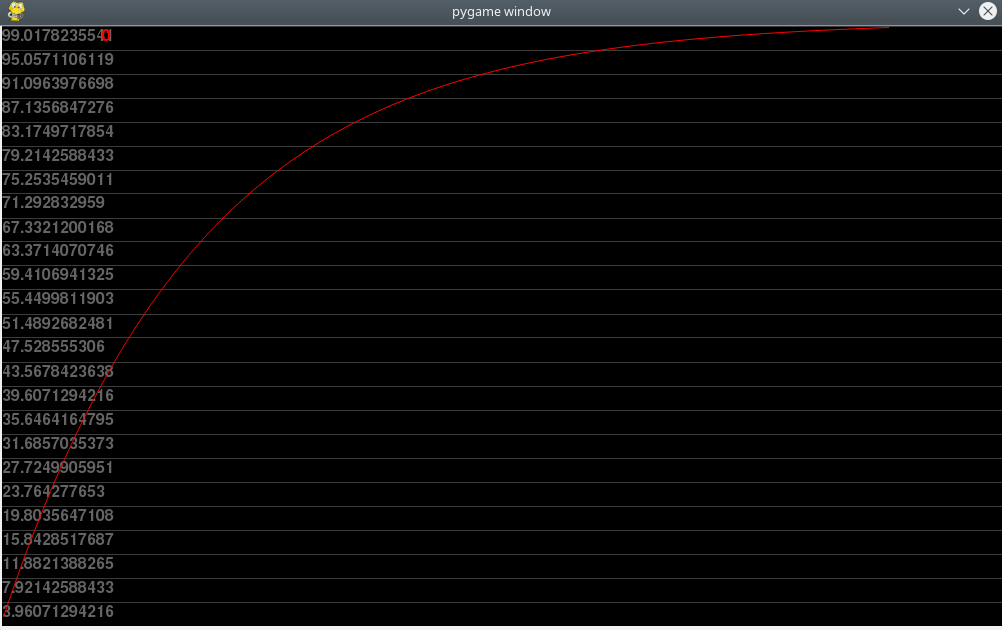
\includegraphics[width=0.7\textwidth]{graph}
\caption{Data visualisation on the PC.}
\label{fig:graphpy}
\end{figure}

%\todo[inline]{Présentation du script de Ken}




% ########   #########  #########  ##         #########  ##    ##   ########     #####    ##      ##
% ##     ##  ##         ##         ##         ##          ##  ##       ##      ##     ##  ###     ##
% ##     ##  ##         ##         ##         ##           ####        ##      ##     ##  ## ##   ##
% ########   ######     ######     ##         ######        ##         ##      ##     ##  ##  ##  ##
% ##   ##    ##         ##         ##         ##           ####        ##      ##     ##  ##   ## ##
% ##    ##   ##         ##         ##         ##          ##  ##       ##      ##     ##  ##     ###
% ##     ##  #########  ##         #########  #########  ##    ##   ########     #####    ##      ##


\section{Methodology}
Before starting such a project, you will have to think about the order of your actions.

It is strongly advised to start by reinterpreting the specifications in the form of a functional block diagram including the basic features of the project.
For each of these features, isolate the peripherals to use and make a schematic diagram of your algorithm.

Once done, implement the project bloc by bloc.
Start with a simple feature such as the command of the fan speed, then complete the rest of the project piece by piece.

Don't code anything too specific to a feature~: remember that the different parts of your algorithm will have to interact with each others.
It might be beneficial to start by implementing the interfaces with the different blocks.
For instance, by coding a function that modify the fan speed.

The purpose behind this project is to program a system while understanding well what you are doing~: no need to go too fast~!



% ##       ##  #########   #######   ##     ##  ########   #########
% ###     ###  ##         ##     ##  ##     ##  ##     ##  ##
% ## ## ## ##  ##         ##         ##     ##  ##     ##  ##
% ##  ###  ##  ######      #######   ##     ##  ########   ######
% ##       ##  ##                ##  ##     ##  ##   ##    ##
% ##       ##  ##         ##     ##  ##     ##  ##    ##   ##
% ##       ##  #########   #######    #######   ##     ##  #########


\section{Temperature measurement}

As mentioned above, the temperature measurement is carried out by means of a platinum resistance traversed by a current of $ 1 mA $.
The electronic diagram is given in the figure~\ref{fig:mes-temp}.

\begin{figure}[H]
\shorthandoff{:!;}
\center
	\subfloat[\label{fig:mes-temp-ampop}]{%
		\parbox[b]{.45\linewidth}{% Embed the content of the subfloat into a parbox to make it wider. Otherwise, the width of the subfloat is set by the width of the table, and so is the caption.
		\center
			\begin{circuitikz}
				\draw
				(0,0) node[op amp] (opamp) {}
				(3,0) node[npn] (npn) {}
				(opamp.out) --(npn.base)
				(npn.collector) to[vR=Pt100] +(0,2) to [short, -o] +(1,0) node (A) {}
				($(npn.collector)+(0,2.5)$) node (vdd) {5V}

				(npn.collector) to [short, -o] +(1,0) node (B) {}
				(A) to[open, v^=$V_{mes}$] (B)

				(npn.emitter) to[short] +(0,-0.5) node(C) {}
				(C) to[R=$R_1$] +(0,-2) node [ground] {}
				($(C)+(0.01,0)$) -| (opamp.+)% For some reason, putting "(C) -| (opamp.+)" leaves a horizontal gap between C and the wire.
				;
			\end{circuitikz}
		}
	}
	\subfloat[\label{fig:mes-temp-current-source}]{%
		\parbox[b]{.45\linewidth}{%The [b] sets the content to be positioned at the bottom of the box.
		\center
			\begin{circuitikz}
				\draw
				(0,-2) to [vR=Pt100] (0,0)
				(0,-2) to [doohicky, l=$1\ mA$] +(0,-2) node [ground] {}
				(0,0.5) node (vdd) {5V}
				(0,0) to [short, -o] (1,0) node (A) {}
				(0,-2) to [short, -o] (1,-2) node (B) {}
				(A) to[open, v^=$V_{mes}$] (B)
				;
			\end{circuitikz}
		}
	}
\caption{Temperature measurement with a Pt100 resistor.}
\label{fig:mes-temp}
\shorthandon{:!;}
\end{figure}

The combination ampli-op + transistor  can be seen as a controllable current source (figure~\ref{fig:mes-temp-current-source})~: by maintaining the tension on $R_1$ with the virtual zero, we maintain simultaneously the current flowing through the resistor.
Since the same current flows through the Pt100, its tension becomes linearly dependent to the temperature.

This measure has two flaws~: not only it is not referenced to the mass, but it is also of low amplitude.
You will therefore, use a a differential amplifier to amplify the tension and to reduce the common mode tension of around $5~V$.

By using an ampli-op INA128 (datasheets are in the appendix), you will have to mount a circuit on a protoboard to acquire the tension and to adapt it to the input voltage of the dsPIC ADC ($0~V$ -- $3.3~V$).




% ##     ##  #########  ##         ########    #######   #########
% ##     ##  ##         ##            ##      ##     ##  ##
% ##     ##  ##         ##            ##      ##         ##
% #########  ######     ##            ##      ##         ######
% ##     ##  ##         ##            ##      ##         ##
% ##     ##  ##         ##            ##      ##     ##  ##
% ##     ##  #########  #########  ########    #######   #########

\section{Power supply of the propeller}\label{sec:helice}
The dePIC doesn't supply enough power for the fan, a power circuit need to be added.
We will use a switching amplifier, those provide a square wave as output instead of a continuous signal.
Its schematics is illustrated on figure~\ref{fig:alim-moteur}.

% \missingfigure[figwidth=\textwidth]{Alimentation moteur}
\begin{figure}[H]
\center
\shorthandoff{:!;}
\begin{circuitikz}
	\draw
	(1,0) node [nmos] (nmos1) {}%anchors are drain, source and gate.
	(1,1.5) node [pmos] (pmos1) {}% 1 = bottom pair
	(1,5) node [nmos] (nmos2) {}% 2 = top pair
	(1,6.5) node [pmos] (pmos2) {}
	(pmos2.source) node[above] () {5V}%Between parenthesis should be the label of the node. Don't any, here.
	(nmos2.source) node [ground] () {}
	(pmos1.source) node[above] () {5V}
	(nmos1.source) node[ground] () {}

	($(nmos2.drain)-(2,0)$) node [left]() {IN1} to [short, -*] +(1,0) node (A) {} -| (pmos2.gate)
	(A) -| (nmos2.gate)

	($(nmos1.drain)-(2,0)$) node [left]() {IN2} to [short, -*] +(1,0) node (B) {} -| (pmos1.gate)
	(B) -| (nmos1.gate)

	(pmos2.drain) to [short] +(3,0) to [twoport,t={Moteur}, bipoles/twoport/height=1.5] +(0,-4) |- (pmos1.drain)
	;
\end{circuitikz}
\shorthandon{:!;}
\caption{Power supply of the motor.}
\label{fig:alim-moteur}
\end{figure}

Each branch of the converter can be seen as a MOS inverter~: when the command is in high state, the bottom transistor is short-circuited while the top transistor is an open circuit.
The difference with classical logic circuit is that the transistors are able to provide higher currents.

The advantage of this system compared with a classical amplification is that it as a high efficiency.
As a first approximation, no power is dissipated in the switches, the power supply efficiency is near from 100~\%.
An additional input named \textit{INHIB}, not represented on the figure, makes possible to deactivate the power supply.

The command of the power amplifier is made with square waves.
Several definitions associated with those waves are illustrated on figure~\ref{fig:square-wave}~:
% \missingfigure[figwidth=\textwidth]{Figure onde carée avec temps de montée et de descente.}
\begin{figure}[H]
\center
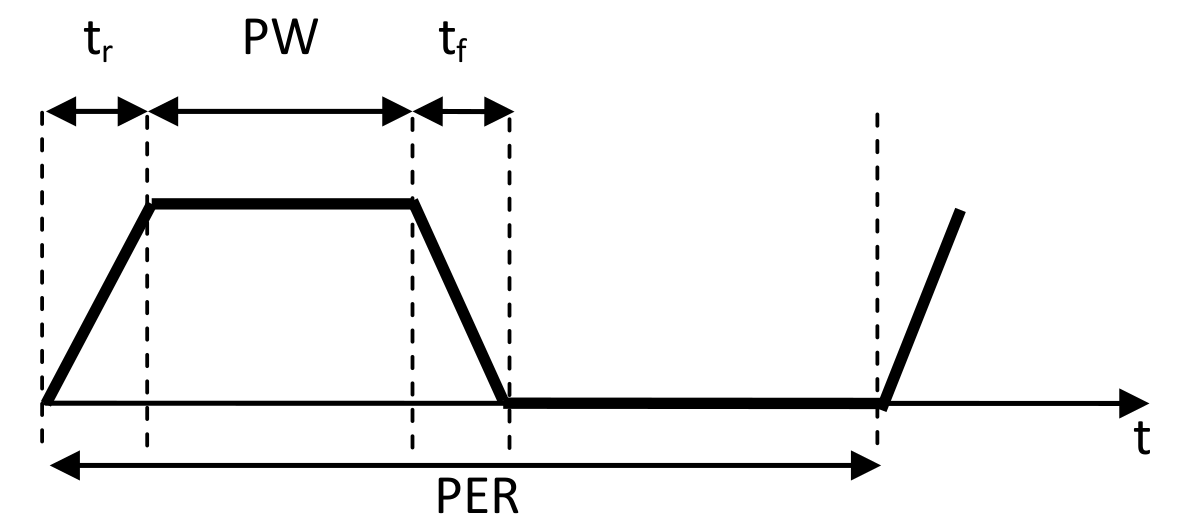
\includegraphics[width=0.6\textwidth]{square-wave}
\caption{Square wave.}
\label{fig:square-wave}
\end{figure}

The different characteristic times are as follows~:
\begin{itemize}
	\item $PW$~: Pulse Width, time in high state.
	\item $PER$~: signal period.
	\item $t_r$~: Rising time.
	\item $t_f$~: Falling time.
\end{itemize}

In most cases, including this one, the rising and falling time are negligible.

An other characteristic is the duty cycle~: it is defined as \[D = \frac{PW}{PER}\]
It is the proportion of time spent in high state during a period.

The PWM command (\textit{Pulse Width Modulation}) consists of sending constant period square wave to the power circuit.
The mean value of the signal is proportional to the duty cycle.

In this case, the signal is the mean tension applied on the DC motor.
Let's take for instance the command signal provided by the dsPIC on figure~\ref{fig:pwm}~:
% \missingfigure[figwidth=\textwidth]{PWM}
\begin{figure}[H]
\center
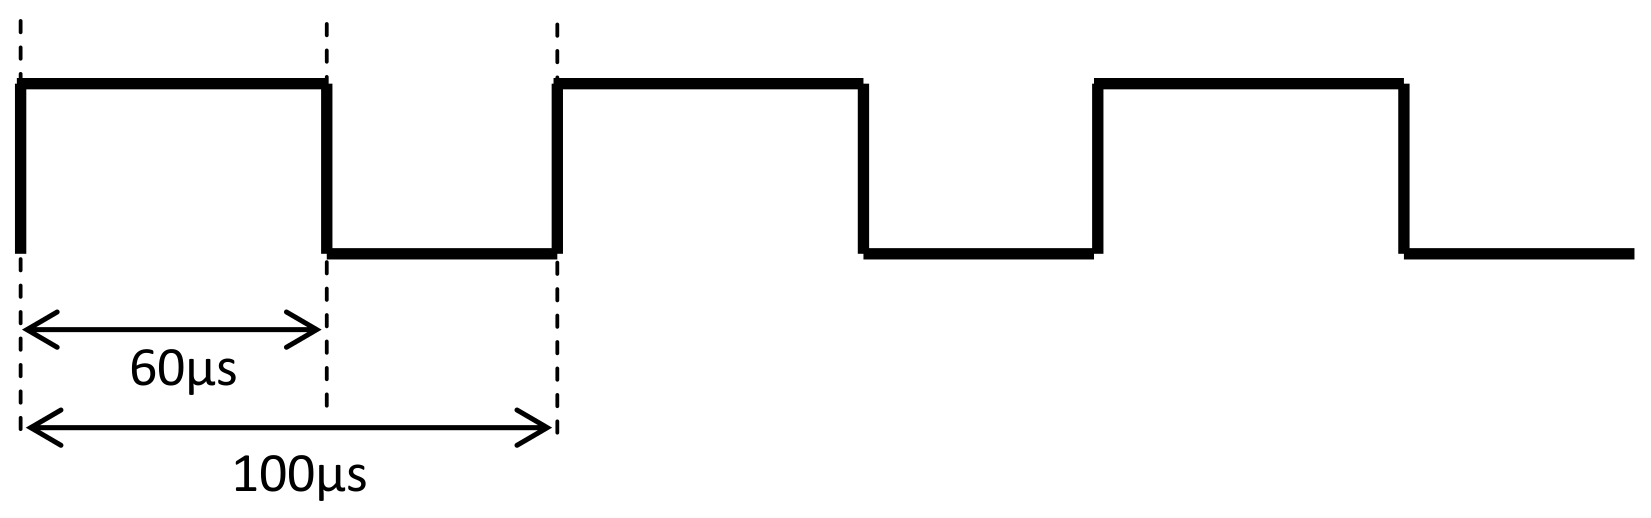
\includegraphics[width=0.7\textwidth]{pwm}
\caption{PWM Signal with a duty cycle of 60~\%.}
\label{fig:pwm}
\end{figure}

This signal is applied on the pin \texttt{IN1} of the motor and pin \texttt{IN2} is connected the ground.

The period is $100 \mu s$ and the duty cycle is $60~\%$.
When the command is in high state, V- is at 0~V and the converter imposes a tension of 5~V to the motor.
When it is not the case, the tension is 0~V.
The mean tension is then $0.6 \cdot 5V  = 3 V$.

\begin{framed}
By playing with the duty cycle, you will be able to modify the propeller speed.
The duty cycle is then the control variable of your regulator.
\end{framed}

The dsPIC has a peripheral to generated PWM waves~: you need to define its period then to configure a specific register to enter the duty cycle.



\end{document}
